\chapter{Experimental Considerations}\label{ch:exp_setup}
%- Start by introducing LCLS\\
%- Introduction to the AMO instrument at LCLS\\
%- Introduction to the LAMP chamber\\
%- Give example experiments to each point
%\section{The X-ray free electron laser LCLS}
%- Describe LCLS more specifically
%\subsection{LCLS pump probe setup}
%- Specifics to our / LCLSs pump probe setup
The experiment described in the present thesis has been performed using the LAMP end-station of the Atomic, Molecular and Optical (AMO) Physics instrument of the Linac Coherent Light Source, which is located at SLAC National Accelerator Laboratory. SLAC was founded in 1962 as Stanford Linear Accelerator Center. The linear accelerator was early on used for high-energy physics experiments and resulted in three Nobel Prizes in Physics \citep{Richter-PRL-1974,Taylor-SLAC-1967,Perl-PRL-1975}. SLAC's research topics broadened in the 1970's and with the Stanford Synchrotron Radiation Project, it became an X-ray user facility in 1974. Meanwhile, the synchrotron source was modernized and is now known as the Stanford Synchrotron Radiation Lightsource (SSRL) and the linear accelerator was repurposed to function as the world's first hard X-ray free electron laser - the LCLS. The LCLS began operations in April 2009 \citep{Emma-2010-NatPho} and the AMO instrument started user operations in October 2009 \citep{Bostedt-2013-JPB}. AMO began operations with the High-Field Physics (HFP) and the CFEL\footnote{Acronym for the Center for Free Electron Laser Science on the DESY campus in Hamburg, Germany.}-ASG\footnote{Short for the Advanced Study Group of the Max Planck Society in Hamburg, Germany.} Multi Purpuse (CAMP) end-station, which was supplied by the Max-Planck Society from Germany. The so-called ``LAMP'' end-station is a successor of the CAMP end-station and was commissioned in September 2013 \citep{Ferguson-2015-JSR}. LAMP has been in use at the AMO instrument since commissioning and the experiment described in this thesis was performed in January 2014\footnote{Experimental identifier at SLAC: \textsc{amoa1214}} in the LAMP end-station of the AMO instrument. My involvement in design discussions, the building, the commissioning, and the operation of the LAMP end-station was a significant effort during my doctoral studies and resulted - at the time of writing - in the publications \citep{Picon-2016-NatComm,Munke-2016-naturedata,Kimberg-2016-FD,Sanchez-Gonzalez-2015-JphysB,Lehmann-2016-PRA,MacDonald-2016-RSI,Gamboa-2016-JI,Bernado-2017-PRB}.\\[1\baselineskip]
%
This chapter is organized as follows; Section \ref{sec:amo-instrument} discusses the the details of the AMO instrument; Section \ref{sec:LAMP-endstation} focuses on the specifics of the LAMP end-station; Section \ref{sec:pnCCD} goes over the pnCCD detector and its geometry; and Section \ref{sec:sample-delivery} centers around relevant aspects of the sample delivery. The chapter ends with Section \ref{sec:TOF-spectrometer} that describes the time-of-flight (TOF) detector for the LAMP end-station.
%
%
%
%\section[The FEE and AMO instrument at the LCLS]{The front end enclosure and the atomic, molecular and optical physics instrument at the LCLS}\label{sec:amo-instrument}
\section{The X-ray beam transport to the LAMP end-station}\label{sec:amo-instrument}
%%%%%%%%%%%%
%- Specifics to AMO\\
%- For example focus studies and KBOs\\
%- Use JSR and previous AMO articles
%%%%%%%%%%%
The AMO instrument is located closest to the undulators of the LCLS at hutch 1. It is designed for soft X-ray photons in the energy range from \SIrange{280}{2000}{\electronvolt} \citep{Ferguson-2015-JSR,Bozek-2009-EPJST}, where the beam divergence is a limiting factor for lower energies and the boron-carbide (B$_{4}$C)-coating on the mirrors leads to absorption above \SI{2000}{\electronvolt}. After the X-ray pulse generation in the undulators of the LCLS, the X-rays are separated from the electron bunch using magnets, and optionally, the X-band transverse deflecting structure (XTCAV) \citep{Behrens-2014-NatCom} can be used to give insight into the kinetic energy and pulse duration of the electron bunch. Prior to entering the Front End Enclosure (FEE) \citep{Moeller-2011-NIMPR}, the electron beam is discarded in the electron dump such that only X-rays continue. In the FEE, the X-rays can be attenuated with either gas or solid attenuators. An X-ray pulse energy monitor, often referred to as a gas detector, measures the pulse energy of a single shot before and after attenuation \citep{Hau-Riege-2010-PRL-2}. Eventually, the X-ray beam is deflected through a mirror system into the desired hutch. To direct the beam to the AMO hutch, the soft X-ray offset mirrors (SOMS) are used. The SOMS are a set of four mirrors, 

where the first two deflect the X-rays to the LCLS instruments that use soft X-rays, namely the AMO and the Soft X-ray (SXR) instrument \citep{Schlotter-2012-RSI,Soufli-2012-AppOpt,Dakovski-2015-JSR}.The third SOMS mirror is a double mirror that either deflects the beam into the AMO or SXR instrument.
\begin{figure}
	\centering
		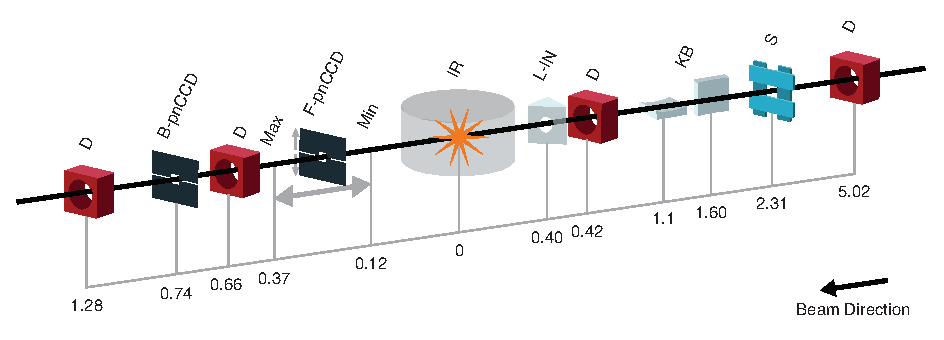
\includegraphics[width=1.00\textwidth]{images/beam_layout.eps}
	\caption[Schematic overview of the AMO beamline instrumentation.]{Schematic overview of the AMO beamline instrumentation in the LAMP configuration. The indicated distances below the schematic items are in meters from the interaction region. As the X-ray beam enters the instrument, it can be visualized on a YAG crystal diagnostics (D). A set of 2 slits (S) cuts the beam in the vertical and horizontal to reduce straylight from the Kirkpatrick-Baez (KB) optics. The differential pumping section of the LAMP end-station houses another YAG crystal diagnostics (D) and an option couple in an optical laser (L-IN) on-axis with the X-rays. The front and back pnCCD (F/B-pnCCD) are located downstream of the IR with further beam viewing options (D). From \citep{Ferguson-2015-JSR}.}
	\label{fig:beam_layout}
\end{figure}
The AMO instrument is versatile in its configuration and three different end-stations have been used so far. In historic order; one, the HFP end-station \citep{Bozek-2009-EPJST,Bostedt-2013-JPB}; two, the diagnostics (DIA) end-station \citep{Bostedt-2013-JPB}; three, CAMP end-station \citep{Strueder-2010-NIMPA}; and four, the LAMP end-station \citep{Ferguson-2015-JSR,Bucher-2016-Unpublished}. Today, the HFP and LAMP end-station can be combined with additional instrumentation, for example, the modernized DIA end-station or the XRSD device (see Section \ref{sec:novel-pump--probe-tech}). As the experiment described in the present work has been performed with the LAMP end-station, we shall focus on that AMO-configuration from here on.\\[1\baselineskip]
%
A schematic overview of the AMO beamline instrumentation in the LAMP configuration can be found in Figure \ref{fig:beam_layout}. As the X-ray beam travels from the FEE to the AMO beamline, it can be viewed with a YAG crystal diagnostic viewer (D). Here the shape and position of the beam can be determined as it is several meters downstream of the SOMS such that a difference of the SOMS angle and position can be determined with sub-millimeter precision. This also reveals the alignment of the beam with respect to several differential pumping apertures that are located in the FEE. Experience shows that the X-rays should be centered to those apertures \citep{Turner-2016-PC}. It is noteworthy already here that the X-ray beam became unstable and the beam's pointing became erratic. The most upstream diagnostic viewer (D) of the AMO instrument was able to detect this jitter such that the linear accelerator could be tuned to correct the erratic pointing. A beamline alignment laser, which is a typical HeNe-laser with low beam divergence, can be coupled into the beamline slightly downstream of the YAG screen\footnote{Not shown in  Figure \ref{fig:beam_layout}} such that it co-propagates with the X-rays. 
%Beamline alignment lasers are invaluable tools to pre-align a system before X-rays are employed. For the described experiment, it was necessary to align the particle jet of the pristine Xe-cluster and the particle jet of the HeXe-cluster to be perpendicular to the X-ray beam (see Figure \ref{fig:Overview-Jetalignment}). 
%In order to perform this alignment, a beamline alignment laser that co-propagates with the X-rays was useful, if not required. 
The X-ray beam then travels through a set of four blades (S), which are often referred to as 4 Jaw slits that can be moved independently to cut into the beam to reduce parasitic scattering\footnote{Parasitic scattering is often referred to as stray light.} originating from the Kirkpatrick-Baez (KB-)mirrors \citep{Kirkpatrick-1948-JOSA}.
%In collaboration with the Single-Particle Initiative \citep{Aquila-2015-StrucDyn}, it was investigated how the blades reduce unwanted scattering. It was found   \citep{SPI-2015-unpublished}
Experience shows that the blades should not cut into the main intensity profile of the beam, but rather conservatively cut into the halo of the beam. This sufficiently reduces parasitic scattering but does not reduce the peak intensity of the X-ray pulse (compare green and blue curve in Figure \ref{fig:Focus-z-scan}).\\[1\baselineskip]
%
The KB-mirrors are a set of two concave mirrors that focus the X-ray beam into the interaction region. The mirrors consist of two \SI{400}{\milli\meter} long silicon (Si) substrates that are coated with boron carbide (B4C). They reflect the X-rays in grazing incidence at \SI{13.85}{\milli\radian} and are sometimes referred to as KB-optics. The first mirror focuses the beam in the horizontal and the second mirror focuses the beam in the vertical. As the mirrors are located at different positions in the horizontal and vertical, they are designed to have a focal length of \SI{1600}{\milli\meter} in the horizontal and \SI{1100}{\milli\meter} in the vertical. Additionally, the mirrors can be bent to change their focusing position along the $Z$-axis\footnote{The LCLS uses a right-handed coordinate system, where the index finger ($Y$-axis) points up and the middle finger ($Z$-axis) points parallel to the X-ray beam.} and the optimal focus can be found and characterized through, for example, the study of time-of-flight (TOF)\index{time-of-flight} mass-spectroscopy \citep{Bucher-2016-Unpublished} and imprint analysis\index{imprint} \citep{Hajkova-2011-SPIE,Chalupsky-2011-NIMPR}, which we will discuss in Section \ref{sec:focus-characterization}. A study of the X-ray focus is necessary to achieve the smallest focus, thereby increasing the intensities at the sample interaction region.
% which is desired in coherent diffractive imaging as thus more photons scatter from the sample and, ideally, to understand the coherent wavefront that creates an image of the particle better.
%
%
%
%
For the experiment in this thesis, the X-ray beam focal size was determined to be $\text{FWHM}\approx \SI{1.5}{\micro\meter}$, with an effective area of $\SI{5}{\micro\meter\squared}$ \citep{Bucher-2016-Unpublished}. The LCLS beam parameters are summarized in Table \ref{tab:beam-params}. The pulse duration was determined through analysis of the electron beam and the delay, $\Delta$t, precision is estimated from geometric considerations of the delay chicane (see also Section \ref{sec:novel-pump--probe-tech}).
\begin{table}
	\centering
		\begin{tabular}{ | l | l | l | }
		\hline
			 & pump beam & probe beam  \\ \hline
			wavelength & \multicolumn{2}{|c|}{1.5 nm} \\ \hline
			mean pulse energy & \SIrange{80}{100}{\micro\joule} & \SIrange{0.8}{1}{\milli\joule} \\ \hline
			X-ray beam FWHM & \multicolumn{2}{|c|}{\SI{\sim 1.5}{\micro\meter}} \\ \hline
			pulse duration & \multicolumn{2}{|c|}{\SI{\sim 25}{\femto\second}} \\ \hline
			delay $\Delta$t precision & \multicolumn{2}{|c|}{\SI{<1}{\femto\second}} \\ \hline
		\end{tabular}
	\caption{Summary of LCLS beam parameters during experiment.}
	\label{tab:beam-params}
\end{table}
%
%
%
\section{The LAMP end-station at the AMO instrument}\label{sec:LAMP-endstation}
%%%%%%%%%%%%%%%%%%
%- Specifics to the LAMP setup\\
%- Use Journal of Synch. Radiation LAMP paper\\
%- I think this can be a longer subsection since a lot of my work went into this.
%%%%%%%%%%%%%%%%%%%
\begin{figure}
	\centering
		\includegraphics[width=0.90\textwidth]{images/AMO-overview-4.eps}
	\caption[Overview of the AMO instrument in the LAMP end-station configuration.]{Overview of the AMO instrument in the LAMP end-station standard configuration. From left to right, the beam propagates through the Kirkpatrick-Baez (KB) optics, the differential pumping (DP) section, the interaction chamber (C1), the front pnCCD chamber (C2-1), the rear pnCCD chamber (C2-2) and finally the diagnostics (DIA) stand. The Xe jet is also shown, including the Parker valve, Xe-source and -skimmer chamber, which are mounted on C1.
%The xenon jet is installed including the manipulator that holds the Parker valve, the Xe source chamber and the Xe skimmmer chamber. The helium jet is not included in this drawing but mounted perpendicular to the Xe jet and the vacuum pumps have not been installed as shown here. For scale, the large, open conflat flanges on the C1 chamber are 12 inch.
}
	\label{fig:LAMP-overview}
\end{figure}
Following the Figure \ref{fig:beam_layout}, the X-ray beam enters the LAMP end-station after the KB mirrors (see also the overview in Figure \ref{fig:LAMP-overview}). LAMP begins with a differential pumping (DP) section that separates the interaction (C1) and detector chambers (C2-1, C2-2) from the KB optics and other upstream beamline instrumentation. The differential pumping section consists of two small tubes, which are pumped with turbo-molecular pumps at neighboring chambers. The tubes are \SI{5}{\milli\meter}, \SI{8}{\milli\meter}, or \SI{10}{\milli\meter} diameter differential pumping apertures (indicated in Figure \ref{fig:c1-ccd-spec}). The DP stage is able to maintain over 4 orders of magnitude pressure difference, for example, the pressure in the C1 vacuum chamber, $p_{\text{C1}}$, may rise to $p_{\text{C1}}=\SI{e-6}{\kilo\pascal}$ as the sample injection starts and the pressure in the KB-optics vacuum tank, $p_{\text{KB}}$, is maintained at $p_{\text{KB}}=\SI{e-10}{\kilo\pascal}$ due to the differential pumping section. The second DP-stage chamber holds a YAG crystal to examine the X-ray beam after the KB optics and a removable laser in-coupling mirror to overlap X-rays with an optical laser or an aperture to reduce parasitic scattering from the differential pumping apertures and upstream elements.\\[1\baselineskip]
\begin{figure}
	\centering
		\includegraphics[width=1.00\textwidth]{images/c1-ccd-spec.jpg}
	\caption{Inside view of the C1 chamber showcasing the interaction region.}
	\label{fig:c1-ccd-spec}
\end{figure}
The beam then travels into the C1 chamber that encloses the interaction region. Before reaching the sample interaction region, the beam is cut by apertures (see Figure \ref{fig:c1-ccd-spec}). The apertures are mounted on encoded stages that are driven by piezoelectric actuators with sub-micron movement precision. The aperture material is silicon nitride ($\text{Si}_{3}\text{N}_{4}$) and has windows with tapered-edges that cut into the X-ray beam. The window-size can be fit to the size of the X-ray beam diameter, which can be estimated using geometric optics. Alternatively, oversized aperture windows can be used to drive one corner of the window on the first aperture stage and the opposite corner on the second stage into the beam, which is sometimes referred to as cornering apertures. As part of this thesis work, an improved aperture system was designed using four aperture blades with tapered edges. These allow full control over the aperture from four directions, thus allowing short aperture alignment times and a more controlled reduction of unwanted effects. For soft X-rays, it is important to note that the flat side of the tapered aperture is facing the beam such that the tapered-edges are facing downstream.\\[1\baselineskip]
%Otherwise unwanted reflections may occur. This aperture system was commissioned in 2015 for diffractive imaging experiments at the AMO instrument.
\begin{figure}
	\centering
		\includegraphics[width=1.0\textwidth]{images/pnCCD-dimensions.jpg}
	\caption[pnCCD detector geometry in the LAMP instrument.]{Side view of the pnCCD detector geometry inside LAMP. The interaction region (IR) is in the center of C1. The beam propagates along the $Z$-axis, where the rear (top) pnCCD is placed \SI{728.53}{\milli\meter} away from the interaction region (original engineering distances). The half detector height is \SI{38.3}{\milli\meter} and results in a scattering angle of $\Theta =$ \SI{4.3}{\degree}. With the gate-valve installed, the front pnCCDs are able to travel along the $Z$-axis from \SIrange{121}{371}{\milli\meter} downstream of the interaction region. The front pnCCDs can be moved along the $Y$-axis and at maximum extension, the outer corners of the front pnCCD detector correspond to a scattering angle of $\Theta=$ \SI{38.1}{\degree}.}
	\label{fig:pnCCD-dimensions}
\end{figure}
In the center of C1, where sample and X-rays interact, a time-of-flight spectrometer can be installed (see Figure \ref{fig:c1-ccd-spec}), which is described in detail in Section \ref{sec:TOF-spectrometer}. The beam then enters the C2-1 chamber through a large gate valve. Here, a variety of distances become relevant for the digital combination of diffraction images from the front and rear pnCCD detectors that are in different planes. This algorithm is discussed in detail in Section \ref{sec:combination-of-images}. Figure \ref{fig:pnCCD-dimensions} shows for this thesis relevant engineering design distances of the pnCCD detectors inside the LAMP instrument including the gate valve. The manufacturing size of the gate-valve along the $Z$-axis is \SI{150.6}{\milli\meter}. The front pnCCD is mounted on a motorized stage and can be moved along the $Z$- and $Y$-axis inside the vacuum. The front-bottom pnCCD module can be set between \SIrange{117.75}{367.75}{\milli\meter} downstream of the center of C1. The front-top pnCCD module is \SI{3.15}{\milli\meter} closer to C1. The maximum extent along the $Y$-axis is \SI{48.3}{\milli\meter} from the beam to the onset of the detector. In this experiment, the front pnCCD modules were in the most rear position and their extent along the $Y$-axis was asymmetric, whereby the front-top pnCCD was \SI{17.3}{\milli\meter} from the beam and the front-bottom pnCCD was \SI{18.9}{\milli\meter}. The distance from the center of C1 to the bottom-rear pnCCD detector module is \SI{731.68}{\milli\meter} and the top-rear pnCCD module is again \SI{3.15}{\milli\meter} closer to C1\footnote{These design distances must be extended by \SI{\sim + 5}{\milli\meter} along the $Z$-axis due to customization during the initial setup of LAMP.}. A set of motorized, in-vacuum stages allow the use of another YAG crystal (D), an optical filter and a B$_{4}$C beam stop just before the rear pnCCD. In this thesis, both pnCCD detectors were used such that another B$_{4}$C beam stop and Yag crystal was mounted on a motorized stage behind the rear pnCCDs to stop the X-rays.
%
%
%
\section{The large area pnCCD detectors}\label{sec:pnCCD}
%%%%%%%%%%%%%%%%%%%%
%- Reuse our work on the LAMP-pnCCD paper\\
%- I think this should be a longer chapter since a lot of my work has gone into this.
%%%%%%%%%%%%%%%%%%%%
The pnCCDs are attractive photon area detectors because of the following four reasons; one, their high quantum efficiency (QE) and good signal to noise ratio; two, their read-out rate is very high -- up to $\SI{200}{\hertz}$; three, their large active areas cover wide scattering angles; and four, the detectors are almost defect free after applying widely-used pixel detector image corrections. pnCCDs are originally designed to be send into space and have found usage in astronomy and material science. The pnCCD detectors have been used first as X-ray diffractive imaging detectors at FLASH and at LCLS, namely in the CAMP instrument. At LCLS, these detectors are mostly used for X-ray diffractive imaging, but have also spectroscopic capabilities, which are demonstrated in the left panel of Figure \ref{fig:pnCCD-histogram}. For this thesis, the pnCCD detectors were used to record diffraction images and are described in detail below.\\[1\baselineskip]
%
\begin{figure}
   \includegraphics[width=0.8\linewidth]{images/pnCCD-detail.png}
    \caption[Geometry of a single pnCCD module.]{Geometry of a single pnCCD module with a detailed view of the beam conveying hole. A single module consists of \SI{1024 x 512}{\pixels}. Each pixel is $\SI{75 x 75}{\micro\meter}$, which results in an active area of \SI{76.8 x 38.4}{\milli\meter}. The chip is surrounded by non-active edges, which are \SI{1.15}{\milli\meter} wide on beam facing edges. The hole reduces the active area on one module by \SI{60 x 22}{\pixels}, or \SI{4.5 x 1.65}{\milli\meter} and allows the beam to propagate through a \SI{2.4 x 1.7}{\milli\meter} hole.}
\label{fig:ccd-detail}
\end{figure}
Let us begin by describing the chip geometry \citep{Bucher-2016-Unpublished}. Each front or rear pnCCD detector is made out of two modules. Figure \ref{fig:ccd-detail} shows the layout of a single pnCCD module\index{pnCCD!module}. The chip consists of \SI{512 x 1024}{\pixels}. Each pixel has a size\index{pnCCD!pixel size} of \SI{75 x 75}{\micro\meter}, so the area that the detector covers is \SI{38.4 x 76.8}{\milli\meter}. To allow the FEL beam to travel through the instrument, each module has a rectangular region cut out in the middle of the center edge. On a single module this area is \SI{4.5 x 1.65}{\milli\meter} and for the whole detector this ``hole'' has the dimensions \SI{4.5 x \sim 4.5}{\milli\meter}. The rear pnCCD position has been chosen such that the pnCCD hole slightly oversizes the diverging FEL beam, when the focus is in the middle of the C1 chamber. The borders of each module are insensitive to photons over a width of \SI{1.15}{\milli\meter} and \SI{1.10}{\milli\meter} at the borders of the hole. To minimize the overall detector area that is insensitive to photons, the two pnCCD\index{pnCCD} modules are mounted such that the non sensitive areas overlap. As a result of that, each top module is \SI{3.15}{\milli\meter} closer to the interaction region than each bottom module. The effective gap that is seen in the laboratory frame images between each top and bottom module measures \SI{16}{\pixels} or \SI{\sim 1.2}{\milli\meter}.\\[1\baselineskip]
%
The pnCCD chip is read out with a custom CMOS multichannel Analog MultiplEXer (CAMEX)\index{pnCCD!CAMEX}. Eight CAMEX are installed on each pnCCD module (indicated on top and bottom of Figure \ref{fig:ccd-detail}). The CAMEX performs two interesting functions; one, instead of reading out every pixel sequentially, it can read-out $128$ pixel rows in parallel enabling pnCCD image read-out rates of up to \SI{200}{\hertz}; two, it pre-amplifies the photon signal through a set of gain amplifiers.
% and three, it converts the signal to an analog output. The analog output containing the image information is converted to a digital signal and stored by the LCLS Data Acquisition (DAQ)\index{pnCCD!Data Acquisition} in the LCLS psana\index{psana} network, where it is accessible for analysis (see Section \ref{sec:LCLS-computing}).\\[1\baselineskip]
\begin{table}%[h!]
\centering
\begin{tabular}{ |c c c c |}
 \hline
 Key & relative  & approx.  & max. photons \\ 
     &   gain    & ADU/keV  & per pixel  \\
 %a & b & c & d & e \\
 %[0.5ex] 
 \hline
 1 & $1/256$ & 5 & 1100  \\
 2 & $1/128$ & 10 & 640   \\
 3 & $1/64$ & 20 & 320   \\
 4 & $1/16$ & 79 & 80  \\
 5 & $1/4$ & 316 & 20  \\
 6 & $1$ & 1250 & 5  \\
 \hline
\end{tabular}
\caption[pnCCD gain modes and typical ADU values at 1k eV photons.]{Typical generated ADU values and dynamic range using 1k eV photons at all pnCCD gain settings. It is a valid approximation to linearly extrapolate to other photon energies.}
\label{tab:gain-modes}
\end{table}
Different gain modes\index{pnCCD!gain} can be used to be more sensitive to photons in high gains or to store more photon signal in lower gains.
The following considerations are useful when combining detectors of different gain settings or arbitrary detector unit (ADU) generation. Table \ref{tab:gain-modes} shows information about the pnCCD gain settings and ADU generation. 
%The different gain amplifications are applied through the CAMEX.
Gain $\tfrac{1}{1}$ is the highest gain and $\tfrac{1}{256}$ is the lowest gain. As one steps from highest to lower gains, e.g., from $1$ to $\tfrac{1}{64}$, the ADU value creation per photon goes with that fraction in good approximation.\\[1\baselineskip]
%Hence, going to lower gains reduces the signal-to-noise ratio but more photon signal can be stored.
%Note, that the table shows typical operating values using $1$ keV photons and that the ADU value creation is dispersive.
%
A for the experiment useful consideration is the quatum efficiency of the pnCCD chip at various wavelengths. The pnCCD is ``back illuminated'' and the entrance windows are coated with \SI{50}{\nano\meter} aluminum to reduce their sensitivity to optical light. For the soft X-ray operating range at the AMO instrument of \SIrange{280}{2000}{\electronvolt}, this alluminum coating attenuates the X-rays only slightly and the detectors maintain a quantum efficiency of \SI{\sim 90}{\percent} \cite{Strueder-2010-NIMPA}. At the AMO instrument, it is thus possible to linearly estimate the generated ADU values from elastic scattering at various photon energies, for example, a \SI{1}{\kilo\electronvolt} photon will generate approximately \num{1250} ADU in highest gain (compare Table \ref{tab:gain-modes}) and a \SI{1.5}{\kilo\electronvolt} photon will generate approximately \num{1750} ADU in highest gain (compare Figure \ref{fig:pnCCD-histogram}). Therefore, the in this thesis used \SI{837}{\electronvolt} photons approximately generate \num{\sim 1087} ADU. For completness, it should be noted that the pnCCDs can be optionally mounted with an Al-filter in front of the entrance windows to reduce effects of optical or infra-red laser light, which were not mounted in this experiment. However, there is an Al-filter mounted on the opposite side of the entrance windows that attenuates scattering from the rear of the chamber and beam stop or so-called ``back scattering''.
%
%
%TBD The thin and unstructured radiation entrance windows have a high quantum-efficiency from the infra-red (IR) to soft X-ray wavelength range. In order to avoid unwanted scattering, the photon entrance windows are located at the back of the detector, thus facing upstream of LCLS, and are coated with \SI{50}{\nano\meter} aluminum to reduce their sensitivity to optical light. This aluminum coating does attenuate the soft X-rays at AMO slightly but the detectors maintain a quantum efficiency of \SI{\sim 90}{\percent}. At AMO, it is thus possible to linearly extrapolate the generated ADU values to other photon energies, for example, a \SI{1.5}{\kilo\electronvolt} photon will generate approximately \num{1750} ADU in highest gain (compare Figure \ref{fig:pnCCD-histogram}). The in this thesis used \SI{837}{\electronvolt} photons will approximately generate \SI{\sim 1087}{\electronvolt}. There is also an optical aluminum filter mounted from the front of the chip, thus facing downstream of LCLS, to drastically reduce wrongly directed scattering.
%
%
%
\section{Sample delivery}\label{sec:sample-delivery}
%\subsection{Xe - cluster}
%- I can probably recycle the usual here
%\subsection{He - cluster}
%- Experimental setup\\
%- Info from Andrey probably needed
%\subsection{HeXe - cluster}
%- Experimental setup\\
%- Info from Andrey probably needed
\begin{figure}
	\centering
		\includegraphics[width=1.00\textwidth]{images/amoa1214-querschnitt.eps}
	\caption[Sideview of double sample jet configuration.]{Downward view of a slice through the interaction region in C1 of the experimental setup. The purple arrow indicates the xenon gas flow, the orange arrow indicates the helium gas flow.}
	\label{fig:Overview-Jetalignment}
\end{figure}
For this experiment, two gas sources are used in order to create single rare-gas clusters; one, a pulsed gas source for high pressure xenon operations at room temperature; and two, a continious gas expansion source for helium operations that is cryogenically cooled. Given the time constraint of performing experiments at the LCLS, both sources are installed in one setup and operate independently, allowing quick sample changes. A schematic setup of the sample environment can be found in Figure \ref{fig:Overview-Jetalignment} and a list of used vacuum pumps can be found in Table \ref{tab:vacuum-table}. The principle of the cluster generation is discussed in Section \ref{sec:homogenous-cluster} and \ref{sec:heterogeneous-cluster}.Experimental aspects of the gas sources and operations is discussed in the following.\\[1\baselineskip]
%Single xenon and helium clusters are produced using the principle of the supersonic gas expansion into a vacuum that is described in Section \ref{sec:homogenous-cluster}. Helium clusters that are doped with xenon are produced through the pickup principle as described in Section \ref{sec:heterogeneous-cluster}. Given the time constraint of performing experiments at the LCLS, both sources are installed in one setup and operate independently, allowing quick sample changes. A schematic setup of the sample environment can be found in Figure \ref{fig:Overview-Jetalignment} and a list of used vacuum pumps can be found in Table \ref{tab:vacuum-table}.\\[1\baselineskip]
\begin{table}
	\centering
\begin{tabular}{ | l | l | l | }
\hline
	\textbf{Chamber} & \textbf{Turbomolecular pump mod.} & \textbf{Roughing pump mod.} \\ \hline
	Xenon source & 4x Leybold Turbovac TMP 361 & \multirow{4}{*}{adixen ACG600} \\ 
	Xenon skimmer & 2x Leybold Turbovac Mag W 300 P &  \\ 
	Helium source & 2x Leybold PK-S 1300 & \\ 
	Helium skimmer & 2x Pfeiffer HiPace 300 & \\ \hline
	LAMP C1 & 1x Pfeiffer HiPace 700 & \multirow{2}{*}{adixen ACP 120G} \\ 
	LAMP C2-1 & 4x Pfeiffer TC 400 & \\ \hline
\end{tabular}
\caption[Installed vacuum pumps in the experiment.]{Installed vacuum pumps per chamber in the experiment.}
\label{tab:vacuum-table}
\end{table}
The AMO cluster source, which produces xenon clusters, consists of a Parker-Hannifin Series 99\footnote{Series 99 is at the time of writing not produced/advertised as a straight, in-line pulsed valve anymore.} pulsed valve using a solenoid with a custom manufactured conical copper nozzle, two vacuum chambers to mount two skimmers, a slit that is adjustable through a piezoelectric motor, and several vacuum pumps. It is a well-characterized source that was used extensively in the past \citep{Ferguson-2016-SciAdv,Ferguson-2015-JSR,Gorkhover-2012-PRL,Gorkhover-2016-NatPho,Rupp-2014-JCP}. The pulsed solenoid valve (see Figure \ref{fig:parker-valve}) is controlled with a Parker-Hannifin Iota One pulsed-valve driver. The valve driver applies a current to the solenoid, a magnetic cylinder with the attached poppet actuates and opens the valve. After the TTL signal from the driver ends, the valve closes again. The valve's opening time is set to 1 ms and repetition rates of up to $30$ Hz can be set at a xenon reservoir pressure range of \SIrange{100}{2000}{\kilo\pascal}. The pulsed valve heats up substantially during operations and due to abrasion, the vespel poppet is replaced every \SI{\sim 60}{\hour} of operating time, or as needed to prevent a leakage from the gas source. The nozzle has a $\SI{200}{\micro\meter}$ opening diameter and an opening half angle of \ang{4}. It is clamped to the Parker valve using an indium gasket to seal. Two skimmers with an opening of 1 mm diameter and an adjustable piezo-skimmer have been installed to define the gas jet. The adjustable slit is formed by two razor blades and the slit width is adjusted through a piezo motor by applying a voltage, $U$, from \SIrange{0}{10}{\volt}. At $U=$ \SI{8}{\volt}, the slit is virtually closed, allowing only one cluster in the slit at a time, which is called the \textit{single cluster regime}. The excess gas in the source and skimmer chambers is removed by turbo-molecular pumps that are connected to roughing pumps (see Table \ref{tab:vacuum-table}). Ultimately, these chambers reduce the gas load of C1 chamber and the pressure, $p_{\text{IR}}$, of the interaction region settles are $p_{\text{IR}}\leq \SI{e-3}{\pascal}$.\\[1\baselineskip]
\begin{figure}
	\centering
		\includegraphics[width=1.00\textwidth]{images/parker-valve.jpg}
	\caption[Schematic of the Parker-Hannifin Series 99 valve.]{Schematic of the Parker-Hannifin Series 99 pulsed in-line valve and custom copper nozzle. The nozzle is clamped to the pulsed valve using an indium gasket to seal. The vespel poppet is attached to the magnetic cylinder and closes the valve. If a current is run through the solenoid, the valve actuates and opens. Adapted from \citep[\href{http://creativecommons.org/licenses/by-nc/3.0/us}{\ccbync}]{Ferguson-2016-PhD}.}
	\label{fig:parker-valve}
\end{figure}
The helium source along with the xenon doping unit and the skimmers is depicted in Figure \ref{fig:Overview-Jetalignment}. Helium droplets are produced in a continuous free gas expansion using an electron microscope diaphragm as nozzle (Plano A0200P) that has a \SI{5}{\micro\meter} orifice and an orifice channel length of \SI{\sim 2}{\micro\meter} \citep{Gomez-2011-JCP}. The nozzle is cooled to cryogenic temperatures $\text{T}= \SI{5.8}{\kelvin}$ using a Sumitomo cold-head. The particle beam is defined by a first \SI{0.5}{\milli\meter} and a second \SI{1}{\milli\meter} diameter skimmer. As explained above, an adjustable slit system allows the definition the gas jet to single helium droplets. A doping unit is installed in the skimmer chamber of the helium source. It is a separate, smaller chamber in the skimmer chamber, where He-clusters can traverse through two smaller holes on each side. So, the gas load from the doping unit is mostly confined, which allows locally increasing the pressure of xenon to $\leq \SI{0.3}{\pascal}$. The pressure is manually controlled using a leak valve. As schematically shown in Figure \ref{fig:pickupPrinciple}, the partial helium pressure is determined with a residual gas analyzer (RGA) opposite the helium source in the chamber that contains the AMO cluster source. The RGA pressure reading is used to determine the depletion of the helium clusters through the pickup of xenon atoms. A thorough alignment of the sources is necessary to overlap the particle beams such they traverse through all skimmers.%A summary of the alignment with a telescope and alignment laser is condensed in appendix \ref{sec:source-alignment}.
%
%
%
\subsection{Sample jet timing at LCLS}\label{sec:jet-timing}
%%%%%%%%%%%
% - explain timing
%%%%%%%%%%%%%%
\begin{figure}
	\centering
		\includegraphics[width=1.00\textwidth]{images/LCLS-timing-schematic.png}
	\caption{Schematic of LCLS EVR timing system.}
	\label{fig:LCLS-EVR-timing}
\end{figure}
Pulsed gas jets such as the one using the Parker solenoid valve require an electric trigger to open the valve. At LCLS, an event generator sends a fiducial, i.e., a clock signal with \SI{360}{\hertz}, and several event codes, e.g., at 120 Hz, to an event receiver (EVR) over a fiber network with a \SI{10}{\pico\second} precision \citep{Krejcik-2007-DIPAC}. The EVR processes these signals and supplies triggers to the components with a specific delay to an event code (EC). Figure \ref{fig:LCLS-EVR-timing} schematically illustrates the timing system. Following the schematic, the process starts with a fiducial and an event code, e.g., EC 140, is delayed by a time of event code x ($TECx$). After a certain time of the fiducial a LCLS pulse arrives. At the AMO instrument, this time\footnote{Times are in nanoseconds (ns) and in a format to comply with the LCLS interface.} is $t_{\text{AMO}}\approx$ \SI{893000}{\nano\second}. Each event code x has a slight variation in arrival time, $TECx$, with respect to the initial fiducial, as the timing signal is clocked with \SI{120}{\mega\hertz}, i.e., \SI{8.4}{\nano\second}. The LCLS control system automatically corrects for different $TECx$ by internally correcting the delay to a reference time $t_{\text{REF}}$ that corresponds to EC 140. EC 140 has a \SI{120}{\hertz} repetition rate and occurs only when an X-ray pulse is present. The reference time is artificially set to $t_{\text{REF}}=$ \SI{100000}{\nano\second}. We can gather the above considerations to establish a delay time to trigger a sample jet to coincide with a LCLS pulse. We note it as
\begin{equation}
t_{\text{delay}} = t_{\text{AMO}} - t_{\text{gas flight time}},
\label{eqn:sample-jet-delay-time}
\end{equation}
with $t_{\text{delay}}$ being the delay value for the LCLS EVR control system and $t_{\text{gas flight time}}$ the flight time of the sample from the gas source to the interaction region. As described in Section \ref{sec:homogenous-cluster} and Reference \citep{Miller-1988-Oxford}, the terminal velocity, $v_{\infty}$, of a sample from a supersonic jet is
\begin{equation}
 v_{\infty} \approx \sqrt{\frac{2\, R\, T_{0}}{m} \left(\frac{\gamma}{\gamma - 1}\right)},
\label{eqn:terminal-velocity}
\end{equation}
with the universal gas constant $R$, the temperature in the stagnation chamber $T_{0}$, and the ratio of specific heats $\gamma = \frac{c_{P}}{c_{V}}$, which is $\gamma = \frac{5}{3}$ for monoatomic gases such as rare-gases. The flight time of a certain gas can then be calculated by measuring the distance, $D$, between the source and the interaction region, thus $t_{\text{gas flight time}}=\frac{D}{v_{\infty}}$. The approach may be extended to approximate flight times of molecules, e.g., using the mass of CO, $m_{\text{CO}}=$ \SI{28}{\amu}, and also to gas mixtures, for example, the mass of a \SI{2}{\percent} xenon-131 and \SI{98}{\percent} helium-4 gas mixture can be estimated using a weighted average according to their relative contributions, thus  $m_{\text{HeXe}} =$ \SI{6.54}{\amu}. As convenience, the Table \ref{tab:terminal-velocities} shows terminal velocities of several rare gases at room temperature.\\[1\baselineskip]
\begin{figure}
	\centering
		\includegraphics[width=0.80\textwidth]{images/gas-jet-flight-times.eps}
	\caption[Event receiver time delay at LCLS for supersonic gas jets.]{$t_{\text{delay}}$ as a function of the gas source distance to the interaction region. Xenon and argon has been used as sample gas in an Even-Lavie pulsed valve. The calculated delay values (solid lines) agree well with the measured delay times (dashed lines) to overlap the onset of the pulsed jet with the laser.}
	\label{fig:LCLS-delay-data}
\end{figure}
Figure \ref{fig:LCLS-delay-data} shows measured and calculated flight times using an Even-Lavie (EL) supersonic gas source\footnote{The EL-valve has the serial no.: EL 5 HRR NO 114.} instead of the earlier described Parker valve. The gas dynamics from an EL-source are similar to a Parker valve, but it has a very well-defined opening time and thus a well-defined gas jet. A typical opening time and the here used one is \SI{22}{\micro\second}, which can be time consuming to trigger properly without knowing $t_{\text{delay}}$. The data show very good overlap of the calculated delay times $t_{\text{delay}}$ from Equation \ref{eqn:sample-jet-delay-time} and the ion yield maximum of the particle beam. The calculated flight times include an error margin, which can also be read as a recommended scan range. While the electric triggering and actual valve opening times may add errors on the microsecond time-scale, uncertainties in temperature and distance from nozzle to the interaction region change delay times drastically.\\[1\baselineskip]
%
\begin{table}
\centering
\begin{tabular}{ | c | c | c | c | c | }
\hline
	\textbf{Sample gas} & \textbf{Helium} & \textbf{Neon} & \textbf{Argon} & \textbf{Xenon} \\ \hline
	$v_{\infty}$ & \SI{1745.5}{\meter\per\second} & \SI{780.6}{\meter\per\second} & \SI{512.0}{\meter\per\second} & \SI{300.0}{\meter\per\second} \\ \hline
\end{tabular}
\caption{Terminal velocities of some rare gases at room temperature.}
\label{tab:terminal-velocities}
\end{table}
%
Very long flight times can occur when heavy gases, such as xenon, are used or long distances, $D$, are necessary. If the flight times $t_{\text{gas flight time}} > t_{\text{AMO}}$ the system has to be delayed onto the next event as negative delays are not possible in the LCLS timing scheme and Equation \eqref{eqn:sample-jet-delay-time} can be rewritten to
\begin{equation}
t_{\text{delay}} = \frac{1}{f_{\text{rr}}} + t_{\text{AMO}} - t_{\text{gas flight time}},
\label{eqn:sample-jet-delay-time-next}
\end{equation}
with $f_{\text{rr}}$ being the repetition rate of the event code.
%
%
%
\section{Time-of-flight mass-spectrometer}\label{sec:TOF-spectrometer}
%%%%%%%%%%%%
%- fundamental aspects to the TOF detector\\
%- I'm hoping on some specific drawings from Timur / LCLS and SIMION simulations from Timur here.
%%%%%%%%%%%%%
An ion time-of-flight spectrometer was used in the interaction region to detect xenon and helium ions. A time-of-flight spectrometer uses electric fields to accelerate ions from the interaction region towards a detector. The detector unit often consists of a micro-channel plate (MCP) that allows recoding an arrival signal and calculating the time-of-flight (TOF) of the ions. The following considerations connect the time-of-flight to ions with a specific \textit{mass-to-charge ratio} \citep{Stephens-1946-APSSpring}.\\[1\baselineskip]
%
In the first stage, the ions are accelerated from the interaction region towards the detector. Here, the electric potential energy is converted into kinetic energy
\begin{align}
q U &= \frac{1}{2}m \left(\frac{d_{1}}{t_{1}}\right)^{2},\\
tof_{1} &= \sqrt{\frac{m}{2qU}}\cdot d_{1},
\end{align}
with $q$ being the elementary charge of the ion, $U$ the voltage difference, $d_{1}$ the distance between the interaction region and spectrometer, $m$ is the mass of the ion, and $tof_{1}$ is the time-of-flight in the acceleration stage. The ions then travel through a drift tube of length $d_{2}$ that is field free. As the velocity remains constant, we can write down
\begin{equation}
tof_{2} = \sqrt{\frac{m}{2qU}}\cdot d_{2},
\end{equation}
with $tof_{2}$ being the time-of-flight in the drift tube. The total flight time can then be written as
\begin{align}
t_{\text{tof}}=tof_{1}+tof_{2}=\sqrt{\frac{m}{2\, q\, U}} \left(d_{1}+d_{2}\right),\intertext{In a typical experiment, all values aside from $m$ and $q$ can be considered constant. Therefore, we may note the time-of-flight in its well known dependency, as}
t_{\text{tof}} \propto \sqrt{\frac{m}{q}}.
\end{align}
%As the spectrometer is a cylindrical system, the time-of-flight denotes the final position on the detector and vice versa. 
%Therefore, $t_{\text{tof}} \propto\sqrt{\frac{m}{q}}$ of the ensemble of ions in the interaction region upon interaction with an X-ray pulse.
In an ideal environment, where atoms become ionized and their kinetic energy, $E_{kin}$, is $E_{kin}=0$, the spectrometer records narrow peaks that are spaced according to their mass-to-charge ratio. However, atomic ions usually start with a kinetic energy, $E_{kin}\neq 0$, such that the time-of-flight is altered and the signal peak structure is broadened. If molecules or clusters become ionized, fragments have additional translational energy resulting from dissociation of a metastable ion measured relative to the center-of-mass, which is often referred to as kinetic energy release \citep{Murray-2013-IUPAC}. This leads to additional broadening of the signal peak structure.
%Atomic ion time-of-flight data typically exhibits a distinct peak structure while the signal from clusters is strongly broadened due to kinetic energy release from collective effects. 
For this thesis, the time-of-flight data is used to measure the level of ionization and kinetic energy release of ions to quantify the degree of sample damage upon irradiation with a LCLS pulse.\\[1\baselineskip]
\begin{figure}
   \includegraphics[width=1.\linewidth]{images/spectrometer.jpg}
    \caption{Drawing of the time-of-flight spectrometer.}
\label{fig:spectrometer-detail}
\end{figure}
The in this experiment used time-of-flight spectrometer is depicted in Figure \ref{fig:spectrometer-detail}. It is a double sided spectrometer for electron and ion detection. %The conical lenses restrict the acceptence of energWith $\pm 5$ keV power supplies, ions can be detected up to kinetic energies of 50 eV with a time-of-flight resolution of 100 ps \citep{Ferguson-2015-JSR}. If only the ion side is used, ions with kinetic energies of up to 100 eV can be detected. The use of $\pm 10$ keV power supplies allows a detection of kinetic energies up to 150 eV. Electrons can be measured up to kinetic energies of 150 eV using $\pm 5$ keV power supplies, 300 eV if only the electron side is used and 400 eV when using $\pm 10$ keV power supplies. Ions and electrons can be detected whether they are emitted in any direction, in other words the spectrometer has a $4\pi$ solid angle collection \citep{Osipov-2013-PC}.
\begin{figure}
   \includegraphics[width=1.\linewidth]{images/simion.jpg}
    \caption[Sideview of the spectrometer showing ion, electron and photon trajectories.]{Sideview of the spectrometer showing ion, electron and photon trajectories upon interaction with LCLS. The image was created with SIMION. From \citep{Osipov-2013-PC}.}
\label{fig:simion}
\end{figure}
A side view of the spectrometer can be found in Figure \ref{fig:simion}. In this schematic, ion, electron and photon trajectories upon interaction with a LCLS pulse have been simulated using SIMION. A conical lens stack avoids casting a shadow on the pnCCD detectors (top of schematic). The applied voltages in the experiment can be found in Table \ref{tab:tof-volategs}. Only ion spectra have been recorded, but in the experiment, the electron side is powered to have unperturbed electric fields across the interaction region.
\begin{table}
\centering
\begin{tabular}{ | c | c || c | c | }
\hline
	\textbf{Ion-side Connection} & \textbf{Voltage in V} & \textbf{El. Side Connection} & \textbf{Voltage in V} \\ \hline
	MCP Front & -2600 & MCP Front & 200 \\ \hline
	MCP Back & 5 & MCP Back & 2200 \\ \hline
	Holder & 200 & Phosphor & 3000 \\ \hline
	Conical lens 70deg & -923 & Holder & 6000 \\ \hline
	Conical lens 53deg & -1393 & Conical lens 70 deg & 500 \\ \hline
	Flat lens \#1 & -1490 & Conical lens 53 deg & 1370 \\ \hline
	Flat lens \#2 & -1564 & Flat lens & 1940 \\ \hline
	Flat lens \#3 & -1639 & Flight tube & 2736 \\ \hline
	Flight tube & -1714 & - & - \\ \hline
\end{tabular}
\caption{Applied voltages to the time-of-flight spectrometer (ion side use only).}
\label{tab:tof-volategs}
\end{table}
%
%
%
\section{Focus characterization}\label{sec:focus-characterization}
A focus characterization is usually performed before X-ray diffractive imaging experiments to optimally focus the X-rays at the desired interaction region. Two focus characterizations methods are described here; one, using a TOF spectrometer; and two, an so-called imprint study.
%
%
%
\subsection{Focus characterization using a TOF spectrometer}
%
\begin{figure}
	\centering
		\includegraphics[width=0.40\textwidth]{images/Focus-z-scan.png}
		\includegraphics[width=0.54\textwidth]{images/Focus-Fractional-Yield.png}
	\caption[Focal spot analysis using a time-of-flight ion spectrometer.]{Left graph: Atomic neon charge state yield from TOF as a function of $Z$-position, relative to optimal focus position $\text{Z}=0$. $Z=0\pm1$ mm is a favorable length for sample injection. Right diagram: Comparison of atomic neon charge state yield from TOF for different cases. Red: Experimental data from October 2009 with 4 blades (S) opened. Green: Experimental data from November 2013 with (S) closed. Blue: Experimental data from November 2013 with (S) opened.}
	\label{fig:Focus-z-scan}
\end{figure}
%
For a focus characterization using a TOF spectrometer, the experimental chamber is usually filled with a well known gas, for example, neon, such that the pressure inside the experimental vacuum chamber is on the order of \SI{e-4}{\pascal}. The TOF spectrometer or the focal point are then moved with respect to each other and ion time-of-flight data is recorded. The left panel in Figure \ref{fig:Focus-z-scan} shows a focus characterization, where a TOF spectrometer was driven along the $Z$-axis on which the X-ray focus was placed. The fractional neon ion yield per charge state is plotted as a function of the spectrometer's $Z$-position. The data shows that a \SI{2}{\milli\meter} region centering around the focal plane at $Z=$ \SI{0}{\milli\meter} is most useful for experiments requiring high X-ray intensities. The right panel of Figure \ref{fig:Focus-z-scan} compares the fractional neon ion yield at the optimal focus position from November \num{2013} \citep{Bucher-2016-Unpublished} to October \num{2009} \citep{Doumy-2011-PRL}. The comparison reveals that high-charge states of neon, for example, $Ne^{8+}$ and $Ne^{9+}$, are less abundant, which can be attributed to the deterioration of the optics over the first years of operations.
%
%
%
\subsection{Focus characterization via imprint study}
%
\begin{figure}
\begin{tabular}{ccc}
  \includegraphics[width=0.25\textwidth]{images/imprints/image0025.jpg} & \includegraphics[width=0.25\textwidth]{images/imprints/image0026.jpg} & \multirow{3}{*}[1.5cm]{\includegraphics[width=0.49\textwidth]{images/imprints/analysis.pdf}} \\
a) & b) & \\[6pt]
 \includegraphics[width=0.25\textwidth]{images/imprints/image0027.jpg} & \includegraphics[width=0.25\textwidth]{images/imprints/image0028.jpg} &  \\
c) & d) & e)
\end{tabular}
\caption[Focal spot analysis via an ex-situ microscope imprint study.]{a)-d) Ex-situ microscope imprint study of a lead tungstate\index{lead tungstate} ($\text{PbWO}_{4}$) sample that was irradiated with single, \SI{1600}{\electronvolt} LCLS pulses at different gas attenuation. e) Non-linearity in Liu plot due to LCLS's super-gaussian beam profile. The approximate FWHM$\approx$ \SI{3.4}{\micro\meter} is determined from the slope of the linear fits, see more in text.}
\label{fig:imprint-study}
\end{figure}
%
In an imprint study, a target, typically a lead tungstate ($\text{PbWO}_{4}$)\index{lead tungstate} window, is placed at the desired interaction region on a motorized stage. The X-ray focus is then moved and for each step at least one X-ray pulse should be shot at the target. The target is then moved slightly since the X-rays point at the same spot and the procedure repeated. This process should be repeated at various X-ray beam attenuation, as we will see below. Figure \ref{fig:imprint-study} shows exemplary data from an imprint study. The $\text{PbWO}_{4}$-target is studied using an optical microscope and typical imprint images are shown in the panel a) to d). Here the target was illuminated with LCLS X-ray pulses at \SI{1600}{\electronvolt} at various transmission values, $T$. The crater sizes varies according to the X-ray fluence and we shall derive in the following the correlation between crater size and the full-width at half-maximum (FWHM).\\[1\baselineskip]
%
Let us describe the energy fluence, E(R), of the X-rays as
\begin{equation}
E(R) = E_{0} e^{\frac{-R^{2}}{2 \sigma^{2}}},
\end{equation}
with the radial coordinate $R$, a characteristic radius $\sigma$, and the peak fluence $E_{0}$. Typically, $\sigma$ stays a constant beam parameter, which is typically set by the optimal focus position of the KB-optics and thus does not affect the crater area. The crater area changes due to varying the peak fluence, $E_{0}$. As $E_{0}$ increases, more and more of the target is irradiated with power densities above the damage threshold such that larger craters form. We can measure the peak fluence, $E_{0}$, through to the pulse energy, $E_{p}$, which is measured with the gas detector. Let us explicitly note their proportional dependency, $E_{0}\propto E_{p}$. Now, we can express the peak fluence more conveniently in terms of the pressure, $p$, in the gas attenuator
\begin{equation}
\log(E_{0}) = \log(E_{\text{in}})+\log(T)= -p \cdot c + \text{const.},
\label{eq:gaussian-beam-imprint}
\end{equation}
with the incident peak fluence at the gas attenuator $E_{in}$ and the transmission $T$. In the gas attenuator, the transmission is $T=e^{-p \cdot c}$ and a constant $c$. The constant $c$ can be derived from \citep{Henke-1993-ADNDT}. For the LCLS attenuator filled with nitrogen gas (N2) over its \SI{4.1}{\meter} length at \SI{1600}{\electronvolt} photon energy, $c\approx$ \SI{74.8127137875}{\pascal}. We can further approximate the crater surface area using a circle. The area then is $\pi r_{0}^{2}$, with the crater radius $r_{0}$. As shown in \citep{Liu-1982-OptLett}, $r_{0}^{2}=2\sigma^{2}log(\frac{E_{0}^{2}}{E_{0}^{1}})$, with $E_{0}^{1/2}$ being the peak fluence at two different attenuation levels. Thus, the slope of a linear fit between the two points $E_{0}^{1/2}$ is $2 \pi \sigma^{2}$. The FWHM is $\text{FWHM}=2\sqrt{2 ln(2)}\sigma$. The right panel of Figure \ref{fig:imprint-study} shows the crater-area as a function of $-log(T)= p \cdot c$, which is often referred to as a Liu's plot. The data points are fitted with two linear fits, which indicate non-linearities that come from a super-Gaussian beam-profile \citep{Chalupsky-2010-OE,Chalupsky-2013-OE}. The FWHM can be determined from the slope of the linear fit at smaller transmissions and is $\text{FWHM}\approx \SI{3.4}{\micro\meter}$ using the exemplary data. The LCLS parameters in the experiment of this thesis are different to the above exemplary data and are summarized in Table \ref{tab:beam-params}.
%
%
%